\documentclass[a4paper,10pt]{article}
\usepackage[utf8]{inputenc}
\usepackage[spanish]{babel}
\usepackage{fancyhdr}
\usepackage{multicol}
\usepackage{geometry}
\usepackage{graphicx}
\usepackage{float}  
\geometry{a4paper, portrait, margin=1in}

\pagestyle{fancy}
\fancyhf{}
\fancyhead[L]{\textbf{Métodos de Optimización}}
\fancyhead[R]{Universidad Nacional del Altiplano - FINESI}
\fancyfoot[C]{\thepage}

\begin{document}
\textbf{Nombre:} Lizbeth Estefany Caceres Tacora.

\textbf{Código:} 230042
\section*{Actividad N° 1: Definición de variable, función y restricciones}
\section*{Variable}

\textbf Es una característica o propiedad que puede cambiar entre diferentes valores y unidades muestrales (Kelmansky, 2009). Estas a su vez son las representaciones que se analizan o miden en unidades estadísticas, los cuales tienen diversos valores de naturaleza cualitativa o cuantitativa (Córdova Zamora, 2022). Como se mencionó, las variables se dividen en dos:

\begin{itemize}
    \item \textbf{Variables cualitativas:} No numéricas, representan cualidades o categorías.
    \item \textbf{Variables cuantitativas:} Numéricas, representan cantidades medibles.
\end{itemize}

Siendo el caso de estudio la presión arterial, la cual se refiere a la presión que ejerce la sangre en los conductos de la aorta y arterias sistémicas (Gerez, 2015). En estadística, esta variable es considerada de tipo cuantitativa, dado que su unidad de medida está dada por mmHg (milímetros de mercurio). Según el National Cancer Institute (s.f.), esta variable incluye dos formas de medición:

\begin{itemize}
    \item \textbf{Presión arterial Sistólica:} Se mide durante el latido del corazón (momento de presión máxima).
    \item \textbf{Presión arterial Diastólica:} Se mide durante el descanso entre dos latidos (momento de presión mínima).
\end{itemize}

Para la medición de la presión arterial (PA): ``La técnica de referencia era la medida en consulta por un médico mediante esfigmomanómetro de mercurio ocluyendo arteria braquial con un manguito y auscultando los ruidos de Korotkoff Fig. 1'' (HTA, 2005).

\vspace{1em}
\begin{figure}[H]
    \centering
    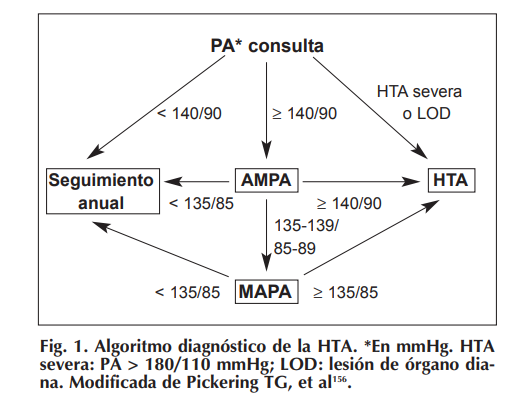
\includegraphics[width=0.75\textwidth]{presion_metodo.png}
    \caption{Técnica para medir la presión arterial.}
    \label{fig:presion}
\end{figure}
\textit{Fuente: HTA, 2005}

\vspace{2em}

\section*{Función}
\textbf Según Martínez (2011), ``La investigación estadística, por sencilla que sea, es una operación compleja, que requiere atender múltiples aspectos, y que genera muy variadas funciones''. De ello se comprende que las funciones sirven para modelar relaciones entre los datos. A su vez, tienden a seguir patrones o predecir valores a partir de los datos.

Un ejemplo de ello se presenta en la investigación \textit{“Modelo matemático de la presión arterial”} de la Universidad Autónoma de Nayarit (2017). En este estudio, se modeló la presión arterial en función de la distancia recorrida, obteniendo las siguientes funciones:

\begin{itemize}
    \item \textbf{Presión Diastólica:} $f(x) = 0.101x + 125.065$
    \item \textbf{Presión Sistólica:} $f(x) = 0.0176x + 82.051$
\end{itemize}

Donde $x$ representa la distancia y $f(x)$ la presión arterial en mmHg. En ambos casos, las funciones son lineales.
\vspace{2em}

En otra investigación relevante, Blanco-Cedres et al. (2003) la función que se obtuvo derivó de los coeficientes de regresión del modelo de estimación de ecuaciones generalizadas. El modelo que se encontró en esta investigación determina cómo varía la presión arterial (sistólica y diastólica) en función de ciertos factores (el índice de masa corporal, el colesterol, la edad, entre otros). Las funciones matemáticas o modelos que se encuentran en este estudio sirven para explicar el comportamiento de la presión arterial en diferentes condiciones o poblaciones.


\vspace{1em}
\begin{figure}[H]
    \centering
    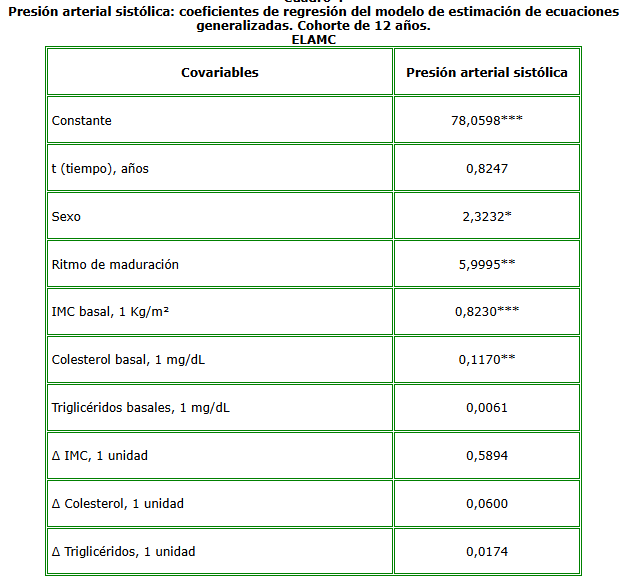
\includegraphics[width=0.75\textwidth]{modelo_blanco_cedres.png}
    \caption{Modelo de presión arterial sistólica según IMC, colesterol y edad, etc}
    \label{fig:modelo_cedres}
\end{figure}
    
\textit {Fuente: Blanco-Cedres et al. (2003)}
\vspace{2em}

En dicho estudio se concluyó que:

\begin{enumerate}
    \item Existe una diferencia promedio de 2,3 mmHg en la presión arterial sistólica entre hombres y mujeres, siendo mayor en varones.
    \item La presión arterial sistólica presentó una asociación positiva y significativa con la maduración temprana, el IMC y el colesterol sérico basal.
\end{enumerate}

\section*{Restricciones}
\textbf Según IBM (2021), ``Una restricción es una regla que se utiliza para fines de optimización''. Es decir, que las restricciones son límites que se imponen sobre los modelos estadísticos para controlar el comportamiento de un proceso, prueba o análisis. Estas reglas pueden ser de varios tipos y se usan en diferentes partes de un estudio o análisis estadsitico, depende de que se quiere lograr.

En cuanto a la presión arterial, estan estan comprendidas en ciertas restricciones, las cuales se presentan a continuación:

\vspace{1em}
\begin{figure}[H]
    \centering
    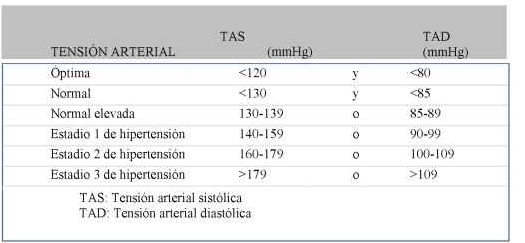
\includegraphics[width=0.6\textwidth]{clasificacion_jnc.png}
    \caption{Clasificación de la hipertensión arterial según el JNC 1997.}
    \label{fig:jnc1997}
\end{figure}
\textit{Fuente: Report of the Joint National Committee, 1977}
\vspace{2em}

\vspace{1em}
\begin{figure}[H]
    \centering
    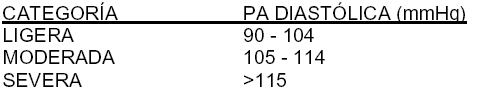
\includegraphics[width=0.6\textwidth]{criterios_oms.png}
    \caption{Criterios de clasificación de la presión arterial según la OMS.}
    \label{fig:oms}
\end{figure}

\textit{Fuente: OMS, citado en HTA (2005)}
\vspace{2em}

\vspace{1em}
\begin{figure}[H]
    \centering
    \includegraphics[width=0.6\textwidth]{clasificación_jncv.png}
    \caption{Clasificación de la presión arterial según el JNC V (1993).}
    \label{fig:jncv}
\end{figure}
\textit{Fuente: JNC V, 1993}

\vspace{2em}

\section*{Referencias Bibliográficas}

\begin{small}
\begin{itemize}
    \item Blanco-Cedres, Lucila, Vásquez, Maura, López-Blanco, Mercedes, \& Macias-Tomei, Coromoto. (2003). Modelización longitudinal de la presión arterial sistólica en función del índice de masa corporal, "ritmo" de maduración, colesterol y triglicéridos en participantes del Estudio Longitudinal de Caracas. \textit{Gaceta Médica de Caracas, 111}(3), 212–219. http://ve.scielo.org/scielo.php?script=sci\_arttext\&pid=S0367-47622003000300006
    \item Córdova Zamora, M. (2022). Estadística descriptiva e inferencial aplicaciones (2ª ed.). DIT. Imp. Edit. Lib. Moshera SRL. ISBN: 978-9972-813-05-4
    \item Gerez, M. (2015). Presión arterial: Anatomo-fisiología. Universidad Nacional de Santiago del Estero. 
    
    https://fhu.unse.edu.ar/carreras/obs/anatomo/presart.pdf
    \item HTA, S. A. (2005). Medida de la presión arterial. \textit{Hipertensión, 22}(Supl 2), 16–26.
    \item IBM. (2021). Tipos de restricciones en DB2 12.1.0. 
    
    https://www.ibm.com/docs/es/db2/12.1.0?topic=constraints-types
    \item Kelmansky, D. M. (2009). \textit{Estadística para todos}. Buenos Aires: Ministerio de Educación-Instituto Nacional de Educación Tecnológica.
    \item Martínez Bencardino, C. (2011). \textit{Estadística básica aplicada} (4.ª ed.). Bogotá: Ecoe Ediciones.
    \item Martín Zurro, A. y Cano Pérez, J.F. (1999). \textit{Atención Primaria}. 4ª ed., Barcelona: Harcourt Brace de España.
    \item National Cancer Institute. (s.f.). \textit{Presión arterial}. 
    
    https://www.cancer.gov/espanol/publicaciones/diccionarios/diccionario-cancer/def/presion-arterial
    \item Report of the Joint National Committee on Detection, Evaluation, and Treatment of High Blood Pressure. \textit{JAMA}, 1977; 237: 255–262.
    \item The Fifth Report of the Joint National Committee on Detection, Evaluation and Treatment of High Blood Pressure (JNC V). \textit{Arch Intern Med}, 1993; 153: 154–183.
    \item Universidad Autónoma de Nayarit. (s.f.). \textit{Modelo matemático de la presión arterial} [Presentación]. 
    
    https://prezi.com/p/bkmbjubdjrxo/modelo-matematico-de-la-presion-arterial/
\end{itemize}
\end{small}

\end{document}
